%===========================================================
% This is the thesis template for the Statistics major at
% Amherst College. Brittney E. Bailey (bebailey@amherst.edu)
% adapted this template from the Reed College LaTeX thesis
% template in January 2019 with major updates in April 2020.
% Please send any comments/suggestions: bebailey@amherst.edu

% Most of the work for the original document class was done
% by Sam Noble (SN), as well as this template. Later comments
% etc. by Ben Salzberg (BTS). Additional restructuring and
% APA support by Jess Youngberg (JY). Email: cus@reed.edu
%===========================================================

\documentclass[12pt, twoside]{amherstthesis}
\usepackage{graphicx,latexsym}
\usepackage{amsmath}
\usepackage{amssymb,amsthm}
\usepackage{longtable,booktabs} %setspace loaded in .cls
\usepackage[hyphens]{url}
\usepackage{hyperref}
\usepackage{lmodern}
\usepackage{float}
\floatplacement{figure}{H}
\usepackage{rotating}
\usepackage{fancyvrb}
% User-added packages:
% End user-added packages

%===========================================================
% BIBLIOGRAPHY FORMATTING

% Next line commented out by CII
%%% \usepackage{natbib}
% Comment out the natbib line above and uncomment the
% following two lines to use the new biblatex-chicago style,
% for Chicago A. Also make some changes at the end where the
% bibliography is included.
%\usepackage{biblatex-chicago}
%\bibliography{thesis}


%===========================================================
% HYPERLINK FORMATTING

% Added by CII (Thanks, Hadley!)
% Use ref for internal links
\renewcommand{\hyperref}[2][???]{\autoref{#1}}
\def\chapterautorefname{Chapter}
\def\sectionautorefname{Section}
\def\subsectionautorefname{Subsection}
% End of CII addition
\usepackage{xcolor}
\hypersetup{
    colorlinks,
    linkcolor={red!50!black},
    citecolor={blue!50!black},
    urlcolor={blue!80!black}
}

%===========================================================
% CAPTION FORMATTING

% Added by CII
\usepackage{caption}
\captionsetup{width=5in}
% End of CII addition

%===========================================================
% TITLE FORMATTING

\renewcommand{\contentsname}{Table of Contents}

\usepackage{titlesec}
%%%%%%%%
% How to use titlesec:
% \titleformat{⟨command⟩}[⟨shape⟩]{⟨format⟩}{⟨label⟩}{⟨sep⟩}
%  {⟨before-code⟩}[⟨after-code⟩]
%%%%%%%%

\titleformat{\chapter}[hang]
{\normalfont%
    \Large% %change this size to your needs for the first line
    \bfseries}{\chaptertitlename\ \thechapter}{1em}{%
      %change this size to your needs for the second line
    }[]

\titleformat{\section}[hang]
{\normalfont%
    \large % %change this size to your needs for the first line
    \bfseries}{\thesection}{1em}{%
     %change this size to your needs for the second line
    }[]

\titleformat{\subsection}[hang]
{\normalfont%
    \normalsize % %change this size to your needs for the first line
    \bfseries}{\thesubsection}{1em}{%
     %change this size to your needs for the second line
    }[]

% \titleformat{\section}[display]
% {\normalfont%
%     \large% %change this size to your needs for the first line
%     \bfseries}{\chaptertitlename\ \thechapter}{20pt}{%
%     \normalsize %change this size to your needs for the second line
%     }


%===========================================================
% DOCUMENT FONT

% \usepackage{times}
% other fonts available eg: times, bookman, charter, palatino


%===========================================================
% PASSING FORMATS FROM RMD --> LATEX

%%%%%%%%
% NOTE: Dollar signs pass parameters between YAML inputs
% in index.Rmd and LaTeX
%%%%%%%%

\Abstract{
The abstract should be a short summary of your thesis work. A paragraph is usually sufficient here.
}

\Acknowledgments{
Use this space to thank those who have helped you in the thesis process (professors, staff, friends, family, etc.). If you had special funding to conduct your thesis work, that should be acknowledged here as well.
}

\Dedication{

}

\Preface{

}

% Formatting R code display
% Syntax highlighting #22
  \usepackage{color}
  \usepackage{fancyvrb}
  \newcommand{\VerbBar}{|}
  \newcommand{\VERB}{\Verb[commandchars=\\\{\}]}
  \DefineVerbatimEnvironment{Highlighting}{Verbatim}{commandchars=\\\{\}}
  % Add ',fontsize=\small' for more characters per line
  \usepackage{framed}
  \definecolor{shadecolor}{RGB}{248,248,248}
  \newenvironment{Shaded}{\begin{snugshade}}{\end{snugshade}}
  \newcommand{\AlertTok}[1]{\textcolor[rgb]{0.94,0.16,0.16}{#1}}
  \newcommand{\AnnotationTok}[1]{\textcolor[rgb]{0.56,0.35,0.01}{\textbf{\textit{#1}}}}
  \newcommand{\AttributeTok}[1]{\textcolor[rgb]{0.13,0.29,0.53}{#1}}
  \newcommand{\BaseNTok}[1]{\textcolor[rgb]{0.00,0.00,0.81}{#1}}
  \newcommand{\BuiltInTok}[1]{#1}
  \newcommand{\CharTok}[1]{\textcolor[rgb]{0.31,0.60,0.02}{#1}}
  \newcommand{\CommentTok}[1]{\textcolor[rgb]{0.56,0.35,0.01}{\textit{#1}}}
  \newcommand{\CommentVarTok}[1]{\textcolor[rgb]{0.56,0.35,0.01}{\textbf{\textit{#1}}}}
  \newcommand{\ConstantTok}[1]{\textcolor[rgb]{0.56,0.35,0.01}{#1}}
  \newcommand{\ControlFlowTok}[1]{\textcolor[rgb]{0.13,0.29,0.53}{\textbf{#1}}}
  \newcommand{\DataTypeTok}[1]{\textcolor[rgb]{0.13,0.29,0.53}{#1}}
  \newcommand{\DecValTok}[1]{\textcolor[rgb]{0.00,0.00,0.81}{#1}}
  \newcommand{\DocumentationTok}[1]{\textcolor[rgb]{0.56,0.35,0.01}{\textbf{\textit{#1}}}}
  \newcommand{\ErrorTok}[1]{\textcolor[rgb]{0.64,0.00,0.00}{\textbf{#1}}}
  \newcommand{\ExtensionTok}[1]{#1}
  \newcommand{\FloatTok}[1]{\textcolor[rgb]{0.00,0.00,0.81}{#1}}
  \newcommand{\FunctionTok}[1]{\textcolor[rgb]{0.13,0.29,0.53}{\textbf{#1}}}
  \newcommand{\ImportTok}[1]{#1}
  \newcommand{\InformationTok}[1]{\textcolor[rgb]{0.56,0.35,0.01}{\textbf{\textit{#1}}}}
  \newcommand{\KeywordTok}[1]{\textcolor[rgb]{0.13,0.29,0.53}{\textbf{#1}}}
  \newcommand{\NormalTok}[1]{#1}
  \newcommand{\OperatorTok}[1]{\textcolor[rgb]{0.81,0.36,0.00}{\textbf{#1}}}
  \newcommand{\OtherTok}[1]{\textcolor[rgb]{0.56,0.35,0.01}{#1}}
  \newcommand{\PreprocessorTok}[1]{\textcolor[rgb]{0.56,0.35,0.01}{\textit{#1}}}
  \newcommand{\RegionMarkerTok}[1]{#1}
  \newcommand{\SpecialCharTok}[1]{\textcolor[rgb]{0.81,0.36,0.00}{\textbf{#1}}}
  \newcommand{\SpecialStringTok}[1]{\textcolor[rgb]{0.31,0.60,0.02}{#1}}
  \newcommand{\StringTok}[1]{\textcolor[rgb]{0.31,0.60,0.02}{#1}}
  \newcommand{\VariableTok}[1]{\textcolor[rgb]{0.00,0.00,0.00}{#1}}
  \newcommand{\VerbatimStringTok}[1]{\textcolor[rgb]{0.31,0.60,0.02}{#1}}
  \newcommand{\WarningTok}[1]{\textcolor[rgb]{0.56,0.35,0.01}{\textbf{\textit{#1}}}}

% Formatting R code: set baselinestretch = 1.5 for double-spacing
\DefineVerbatimEnvironment{Highlighting}{Verbatim}{
  baselinestretch = 1,
  commandchars=\\\{\}}

% Formatting R output display: set baselinestretch = 1.5 for double-spacing
\DefineVerbatimEnvironment{verbatim}{Verbatim}{
  baselinestretch = 1,
  % indent from left margin
  xleftmargin = 1mm,
  % vertical grey bar on left side of R output
  frame = leftline,
  framesep = 0pt,
  framerule = 1.5mm, rulecolor = \color{black!15}
  }

\title{My amazing title}
\author{Your R. Name}
\date{April DD, 20YY}
\division{}
\advisor{Advisor F. Name}
% for second advisor
\altadvisor{Your Other Advisor}
\institution{Amherst College}
\degree{Bachelor of Arts}
\department{Mathematics and Statistics}

% Fix from pandoc about cslreferences?
% https://github.com/mpark/wg21/issues/54
\newlength{\cslhangindent}
\setlength{\cslhangindent}{1.5em}
\newenvironment{CSLReferences}[2]%
  {}%
  {\par}

% Added by CII
%%% Copied from knitr
%% maxwidth is the original width if it's less than linewidth
%% otherwise use linewidth (to make sure the graphics do not exceed the margin)
\makeatletter
\def\maxwidth{ %
  \ifdim\Gin@nat@width>\linewidth
    \linewidth
  \else
    \Gin@nat@width
  \fi
}
\makeatother

% ===========================================
% DOCUMENT SPACING

\setlength{\parskip}{0pt}
% Added by CII

\providecommand{\tightlist}{%
  \setlength{\itemsep}{0pt}\setlength{\parskip}{0pt}}


% ===========================================
% ===========================================
% ===========================================
\usepackage{amsthm}
\newtheorem{theorem}{Theorem}[chapter]
\newtheorem{lemma}{Lemma}[chapter]
\newtheorem{corollary}{Corollary}[chapter]
\newtheorem{proposition}{Proposition}[chapter]
\newtheorem{conjecture}{Conjecture}[chapter]
\theoremstyle{definition}
\newtheorem{definition}{Definition}[chapter]
\theoremstyle{definition}
\newtheorem{example}{Example}[chapter]
\theoremstyle{definition}
\newtheorem{exercise}{Exercise}[chapter]
\theoremstyle{definition}
\newtheorem{hypothesis}{Hypothesis}[chapter]
\theoremstyle{remark}
\newtheorem*{remark}{Remark}
\newtheorem*{solution}{Solution}
\begin{document}

\doublespace
% Everything below added by CII
  \maketitle

\frontmatter % this stuff will be roman-numbered
\pagenumbering{roman}
\pagestyle{fancyplain}
%\pagestyle{fancy} % this removes page numbers from the frontmatter

  \begin{abstract}
    The abstract should be a short summary of your thesis work. A paragraph is usually sufficient here.
  \end{abstract}
  \begin{acknowledgments}
    Use this space to thank those who have helped you in the thesis process (professors, staff, friends, family, etc.). If you had special funding to conduct your thesis work, that should be acknowledged here as well.
  \end{acknowledgments}

  \hypersetup{linkcolor=black}
  \setcounter{tocdepth}{2}
  \tableofcontents

  \addcontentsline{toc}{chapter}{List of Tables}\listoftables

  \addcontentsline{toc}{chapter}{List of Figures}\listoffigures


\mainmatter % here the regular arabic numbering starts
\pagenumbering{arabic}
\pagestyle{fancyplain} % turns page numbering back on

\hypertarget{intro}{%
\chapter{Introduction}\label{intro}}

The field of preventive epidemiology involves the identification of potentially modifiable risk factors that contribute to the burden of disease within human populations. Environmental epidemiology, in particular, considers the effect of environmental exposures --- chemical or otherwise --- which have been increasingly recognized as crucial determinants of human health (Vineis, 2018). Understanding the health effects of exposure to chemical pollutants is especially timely. It has been estimated that human activity releases chemicals at a rate of 220 billion tons per annum (Cribb, 2016). As a result, exposure to low levels of pollutants has become an inevitable peril of daily life. Scholars warn that such conditions of cumulative chronic toxicity pose an acute risk to the wellbeing of humans and our living environment (Naidu et al., 2021). To this, the quantification of such risks through environmental epidemiology studies can prompt critical regulatory action.

Studies concerning chemical pollutants in environmental epidemiology have historically focused on elucidating the effect and mechanisms of single exposures. However, humans are invariably exposed to numerous complex chemical mixtures which together contribute to the progression of adverse health outcomes --- risk assessments of single pollutants likely fail to capture the true consequences of these complex exposures (Heys et al., 2016). Assessing mixtures of chemicals can also have more direct implications for public health interventions. The United States Environmental Protection Agency (U.S. EPA) currently passes regulations for individual pollutants. In practice, though, regulation occurs by controlling the source of pollution, which is responsible for the production of a whole mixture of chemicals with specific joint effects on human health. As a result, the National Academies of Science has advocated for a multipollutant regulatory approach, which is likely to be more protective of human health (Committee on Incorporating 21st Century Science into Risk-Based Evaluations et al., 2017).

Hence, there are clear practical motivations for the development of studies and methodologies that examine the health effects of exposure to co-occurring chemical mixtures, hereafter referred to as exposure mixtures. However, expanding the focus of analysis from one exposure to multiple exposures introduces unique statistical challenges. In addition to the issue of small effect sizes and small sample sizes present in all exposure analyses, multiple exposure analyses must also contend with high-dimensionality, collinearity, non-linear effects, and non-additive interactions (Yu et al., 2022). The classic multiple linear regression framework fails to capture the true effects in this setting. In the past few years, a wide variety of statistical methods have been developed to overcome these challenges (Gibson et al., 2019; Yu et al., 2022), which have been accompanied by a host of comparative simulation studies for general mixture scenarios (e.g., Hoskovec et al., 2021; Lazarevic et al., 2020; Pesenti et al., 2023). However, there is not yet conclusive guidance about the ability of these methods to conduct inference on non-additive interactions between exposures.

The goal of this thesis is to explore the theory of emerging Bayesian regression techniques for quantifying complex interactions between environmental exposures. \textbf{{[}clarify goals{]}}

In an age where anthropogenic actions have radically reshaped the earth, humanistic inquiry can offer critical insights into our place within a rapidly evolving environment. I begin in Chapter 2 by contextualizing this thesis with a brief overview of cultural and social understandings of the topic of environmental exposures. Chapter 3 provides background on X Bayesian methods for analyzing exposure mixtures. Chapter 4 assesses the performance of these methods for conducting inference on non-additive interactions using a simulation study based on \textbf{X}. Chapter 5 explores an application on \textbf{X} data \textbf{{[}TBD{]}}. I conclude with a discussion of the implications of this work for the future study of complex interactions in exposure mixture studies.

\hypertarget{rmd-basics}{%
\chapter{R Markdown Basics}\label{rmd-basics}}

Be careful with your spacing in \emph{Markdown} documents. While whitespace largely is ignored, it does at times give \emph{Markdown} signals as to how to proceed. As a habit, try to keep everything left aligned whenever possible, especially as you type a new paragraph. In other words, there is no need to indent basic text in the Rmd document (in fact, it might cause your text to do funny things if you do).

\hypertarget{lists}{%
\section{Lists}\label{lists}}

It's easy to create a list. It can be unordered like
\begin{itemize}
\tightlist
\item
  Item 1
\item
  Item 2
\end{itemize}
or it can be ordered like
\begin{enumerate}
\def\labelenumi{\arabic{enumi}.}
\tightlist
\item
  Item 1
\item
  Item 2
\end{enumerate}
Notice that I intentionally mislabeled Item 2 as number 4. \emph{Markdown} automatically figures this out! You can put any numbers in the list and it will create the list. Check it out below.

To create a sublist, just indent the values a bit (at least four spaces or a tab). (Here's one case where indentation is key!)
\begin{enumerate}
\def\labelenumi{\arabic{enumi}.}
\tightlist
\item
  Item 1
\item
  Item 2
\item
  Item 3
  \begin{itemize}
  \tightlist
  \item
    Item 3a
  \item
    Item 3b
  \end{itemize}
\end{enumerate}
\hypertarget{line-breaks}{%
\section{Line breaks}\label{line-breaks}}

Make sure to add white space between lines if you'd like to start a new paragraph. Look at what happens below in the outputted document if you don't:

Here is the first sentence. Here is another sentence. Here is the last sentence to end the paragraph.
This should be a new paragraph.

\emph{Now for the correct way:}

Here is the first sentence. Here is another sentence. Here is the last sentence to end the paragraph.

This should be a new paragraph.

\hypertarget{r-chunks}{%
\section{R chunks}\label{r-chunks}}

When you click the \textbf{Knit} button above a document will be generated that includes both content as well as the output of any embedded \textbf{R} code chunks within the document. You can embed an \textbf{R} code chunk like this (\texttt{cars} is a built-in \textbf{R} dataset):
\begin{Shaded}
\begin{Highlighting}[]
\FunctionTok{summary}\NormalTok{(cars)}
\end{Highlighting}
\end{Shaded}
\begin{verbatim}
        speed           dist    
    Min.   : 4.0   Min.   :  2  
    1st Qu.:12.0   1st Qu.: 26  
    Median :15.0   Median : 36  
    Mean   :15.4   Mean   : 43  
    3rd Qu.:19.0   3rd Qu.: 56  
    Max.   :25.0   Max.   :120
\end{verbatim}
\hypertarget{inline-code}{%
\section{Inline code}\label{inline-code}}

If you'd like to put the results of your analysis directly into your discussion, add inline code like this:
\begin{quote}
The \texttt{cos} of \(2 \pi\) is 1.
\end{quote}
Another example would be the direct calculation of the standard deviation:
\begin{quote}
The standard deviation of \texttt{speed} in \texttt{cars} is 5.288.
\end{quote}
One last neat feature is the use of the \texttt{ifelse} conditional statement which can be used to output text depending on the result of an \textbf{R} calculation:
\begin{quote}
The standard deviation is less than 6.
\end{quote}
Note the use of \texttt{\textgreater{}} here, which signifies a quotation environment that will be indented.

As you see with \texttt{\$2\ \textbackslash{}pi\$} above, mathematics can be added by surrounding the mathematical text with dollar signs. More examples of this are in \protect\hyperlink{math-sci}{Mathematics and Science} if you uncomment the code in \protect\hyperlink{math}{Math}.

\hypertarget{including-plots}{%
\section{Including plots}\label{including-plots}}

You can also embed plots. For example, here is a way to use the base \textbf{R} graphics package to produce a plot using the built-in \texttt{pressure} dataset:
\begin{center}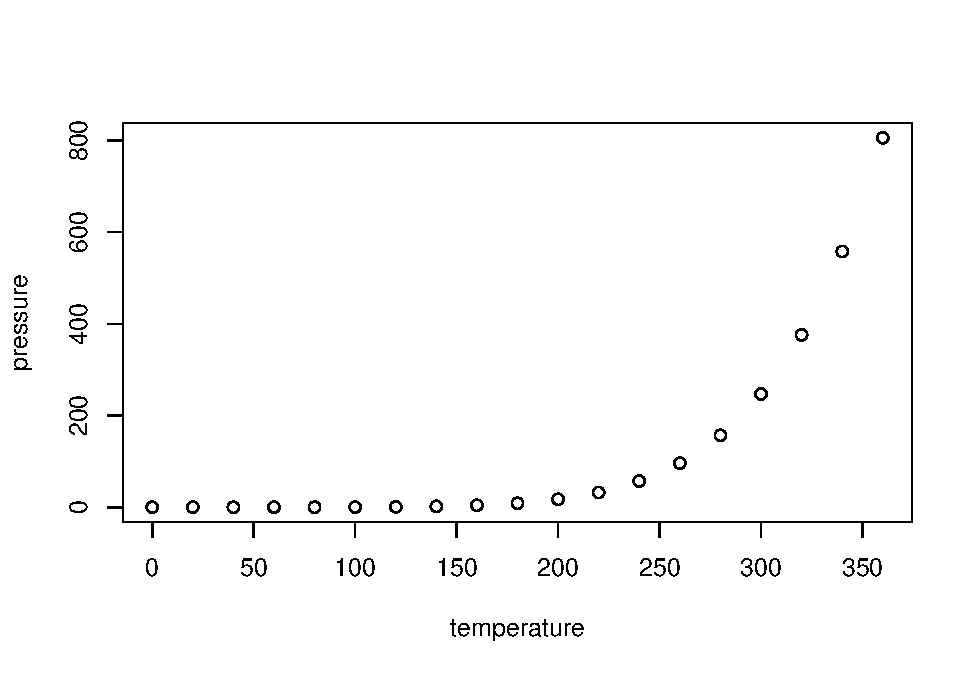
\includegraphics{firstName-lastName_StatThesis_files/figure-latex/pressure-1} \end{center}

Note that the \texttt{echo=FALSE} parameter was added to the code chunk to prevent printing of the \textbf{R} code that generated the plot. There are plenty of other ways to add chunk options. More information is available at \url{http://yihui.name/knitr/options/}.

Another useful chunk option is the setting of \texttt{cache=TRUE} as you see here. If document rendering becomes time consuming due to long computations or plots that are expensive to generate you can use knitr caching to improve performance. Later in this file, you'll see a way to reference plots created in \textbf{R} or external figures.

\hypertarget{loading-and-exploring-data}{%
\section{Loading and exploring data}\label{loading-and-exploring-data}}

Included in this template is a file called \texttt{flights.csv}. This file includes a subset of the larger dataset of information about all flights that departed from Seattle and Portland in 2014. More information about this dataset and its \textbf{R} package is available at \url{http://github.com/ismayc/pnwflights14}. This subset includes only Portland flights and only rows that were complete with no missing values. Merges were also done with the \texttt{airports} and \texttt{airlines} data sets in the \texttt{pnwflights14} package to get more descriptive airport and airline names.

We can load in this data set using the following command:
\begin{Shaded}
\begin{Highlighting}[]
\NormalTok{flights }\OtherTok{\textless{}{-}} \FunctionTok{read.file}\NormalTok{(}\StringTok{"data/flights.csv"}\NormalTok{)}
\end{Highlighting}
\end{Shaded}
\begin{verbatim}
   Reading data with read.csv()
\end{verbatim}
The data is now stored in the data frame called \texttt{flights} in \textbf{R}. To get a better feel for the variables included in this dataset we can use a variety of functions. Here we can see the dimensions (rows by columns) and also the names of the columns.
\begin{Shaded}
\begin{Highlighting}[]
\FunctionTok{dim}\NormalTok{(flights)}
\end{Highlighting}
\end{Shaded}
\begin{verbatim}
   [1] 52808    16
\end{verbatim}
\begin{Shaded}
\begin{Highlighting}[]
\FunctionTok{names}\NormalTok{(flights)}
\end{Highlighting}
\end{Shaded}
\begin{verbatim}
    [1] "month"        "day"          "dep_time"     "dep_delay"   
    [5] "arr_time"     "arr_delay"    "carrier"      "tailnum"     
    [9] "flight"       "dest"         "air_time"     "distance"    
   [13] "hour"         "minute"       "carrier_name" "dest_name"
\end{verbatim}
\begin{Shaded}
\begin{Highlighting}[]
\CommentTok{\# read long paragraph file}
\NormalTok{longtext }\OtherTok{\textless{}{-}} \FunctionTok{readLines}\NormalTok{(}\StringTok{"data/paragraphs.txt"}\NormalTok{)}
\end{Highlighting}
\end{Shaded}
\begin{verbatim}
   Warning in readLines("data/paragraphs.txt"): incomplete final
   line found on 'data/paragraphs.txt'
\end{verbatim}
\begin{Shaded}
\begin{Highlighting}[]
\CommentTok{\# display text as vector}
\NormalTok{longtext}
\end{Highlighting}
\end{Shaded}
\begin{verbatim}
   [1] "Lorem ipsum dolor sit amet, consectetur adipiscing elit,
   sed do eiusmod tempor incididunt ut labore et dolore magna
   aliqua. Ut enim ad minim veniam, quis nostrud exercitation
   ullamco laboris nisi ut aliquip ex ea commodo consequat. "
   [2] ""
   [3] "Duis aute irure dolor in reprehenderit in voluptate
   velit esse cillum dolore eu fugiat nulla pariatur. Excepteur
   sint occaecat cupidatat non proident, sunt in culpa qui
   officia deserunt mollit anim id est laborum."
\end{verbatim}
\begin{Shaded}
\begin{Highlighting}[]
\CommentTok{\# display text as paragraphs}
\FunctionTok{cat}\NormalTok{(longtext)}
\end{Highlighting}
\end{Shaded}
\begin{verbatim}
   Lorem ipsum dolor sit amet, consectetur adipiscing elit, sed
   do eiusmod tempor incididunt ut labore et dolore magna
   aliqua. Ut enim ad minim veniam, quis nostrud exercitation
   ullamco laboris nisi ut aliquip ex ea commodo consequat.
   Duis aute irure dolor in reprehenderit in voluptate velit
   esse cillum dolore eu fugiat nulla pariatur. Excepteur sint
   occaecat cupidatat non proident, sunt in culpa qui officia
   deserunt mollit anim id est laborum.
\end{verbatim}
\begin{Shaded}
\begin{Highlighting}[]
\CommentTok{\# display text without linewidth option specified}
\NormalTok{longtext}
\end{Highlighting}
\end{Shaded}
\begin{verbatim}
   [1] "Lorem ipsum dolor sit amet, consectetur adipiscing elit, sed do eiusmod tempor incididunt ut labore et dolore magna aliqua. Ut enim ad minim veniam, quis nostrud exercitation ullamco laboris nisi ut aliquip ex ea commodo consequat. "
   [2] ""                                                                                                                                                                                                                                        
   [3] "Duis aute irure dolor in reprehenderit in voluptate velit esse cillum dolore eu fugiat nulla pariatur. Excepteur sint occaecat cupidatat non proident, sunt in culpa qui officia deserunt mollit anim id est laborum."
\end{verbatim}
Another good idea is to take a look at the dataset in table form. With this dataset having more than 50,000 rows, we won't explicitly show the results of the command here. I recommend you enter the command into the Console \textbf{\emph{after}} you have run the \textbf{R} chunks above to load the data into \textbf{R}.
\begin{Shaded}
\begin{Highlighting}[]
\FunctionTok{View}\NormalTok{(flights)}
\end{Highlighting}
\end{Shaded}
While not required, it is highly recommended you use the \texttt{dplyr} package to manipulate and summarize your data set as needed. It uses a syntax that is easy to understand using chaining operations. Below I've created a few examples of using \texttt{dplyr} to get information about the Portland flights in 2014. You will also see the use of the \texttt{ggplot2} package, which produces beautiful, high-quality academic visuals.

The example we show here does the following:
\begin{itemize}
\item
  Selects only the \texttt{carrier\_name} and \texttt{arr\_delay} from the \texttt{flights} dataset and then assigns this subset to a new variable called \texttt{flights2}.
\item
  Using \texttt{flights2}, we determine the largest arrival delay for each of the carriers.
\end{itemize}
\begin{Shaded}
\begin{Highlighting}[]
\NormalTok{flights2 }\OtherTok{\textless{}{-}}\NormalTok{ flights }\SpecialCharTok{\%\textgreater{}\%} 
  \FunctionTok{select}\NormalTok{(carrier\_name, arr\_delay)}
\NormalTok{max\_delays }\OtherTok{\textless{}{-}}\NormalTok{ flights2 }\SpecialCharTok{\%\textgreater{}\%} 
  \FunctionTok{group\_by}\NormalTok{(carrier\_name) }\SpecialCharTok{\%\textgreater{}\%}
  \FunctionTok{summarize}\NormalTok{(}\AttributeTok{max\_arr\_delay =} \FunctionTok{max}\NormalTok{(arr\_delay, }\AttributeTok{na.rm =} \ConstantTok{TRUE}\NormalTok{))}
\end{Highlighting}
\end{Shaded}
A useful function in the \texttt{knitr} package for making nice tables in \emph{R Markdown} is called \texttt{kable}. It is much easier to use than manually entering values into a table by copying and pasting values into Excel or LaTeX. This again goes to show how nice reproducible documents can be! (Note the use of \texttt{results="asis"}, which will produce the table instead of the code to create the table.) The \texttt{caption.short} argument is used to include a shorter title to appear in the List of Tables.
\begin{Shaded}
\begin{Highlighting}[]
\FunctionTok{kable}\NormalTok{(max\_delays, }
      \AttributeTok{col.names =} \FunctionTok{c}\NormalTok{(}\StringTok{"Airline"}\NormalTok{, }\StringTok{"Max Arrival Delay"}\NormalTok{),}
      \AttributeTok{caption =} \StringTok{"Maximum Delays by Airline"}\NormalTok{,}
      \AttributeTok{caption.short =} \StringTok{"Max Delays by Airline"}\NormalTok{,}
      \AttributeTok{longtable =} \ConstantTok{TRUE}\NormalTok{,}
      \AttributeTok{booktabs =} \ConstantTok{TRUE}\NormalTok{)}
\end{Highlighting}
\end{Shaded}
\begin{longtable}[t]{lr}
\caption[Max Delays by Airline]{\label{tab:maxdelays}Maximum Delays by Airline}\\
\toprule
Airline & Max Arrival Delay\\
\midrule
Alaska Airlines Inc. & 338\\
American Airlines Inc. & 1539\\
Delta Air Lines Inc. & 651\\
Frontier Airlines Inc. & 575\\
Hawaiian Airlines Inc. & 407\\
\addlinespace
JetBlue Airways & 273\\
SkyWest Airlines Inc. & 421\\
Southwest Airlines Co. & 694\\
US Airways Inc. & 347\\
United Air Lines Inc. & 472\\
\addlinespace
Virgin America & 366\\
\bottomrule
\end{longtable}
The last two options make the table a little easier-to-read.

We can further look into the properties of the largest value here for American Airlines Inc.~To do so, we can isolate the row corresponding to the arrival delay of 1539 minutes for American in our original \texttt{flights} dataset.
\begin{Shaded}
\begin{Highlighting}[]
\NormalTok{flights }\SpecialCharTok{\%\textgreater{}\%} \FunctionTok{filter}\NormalTok{(arr\_delay }\SpecialCharTok{==} \DecValTok{1539}\NormalTok{, }
\NormalTok{                  carrier\_name }\SpecialCharTok{==} \StringTok{"American Airlines Inc."}\NormalTok{) }\SpecialCharTok{\%\textgreater{}\%}
  \FunctionTok{select}\NormalTok{(}\SpecialCharTok{{-}}\FunctionTok{c}\NormalTok{(month, day, carrier, dest\_name, hour, }
\NormalTok{            minute, carrier\_name, arr\_delay))}
\end{Highlighting}
\end{Shaded}
\begin{verbatim}
     dep_time dep_delay arr_time tailnum flight dest air_time
   1     1403      1553     1934  N595AA   1568  DFW      182
     distance
   1     1616
\end{verbatim}
We see that the flight occurred on March 3rd and departed a little after 2 PM on its way to Dallas/Fort Worth. Lastly, we show how we can visualize the arrival delay of all departing flights from Portland on March 3rd against time of departure.
\begin{Shaded}
\begin{Highlighting}[]
\NormalTok{flights }\SpecialCharTok{\%\textgreater{}\%} \FunctionTok{filter}\NormalTok{(month }\SpecialCharTok{==} \DecValTok{3}\NormalTok{, day }\SpecialCharTok{==} \DecValTok{3}\NormalTok{) }\SpecialCharTok{\%\textgreater{}\%}
  \FunctionTok{ggplot}\NormalTok{(}\FunctionTok{aes}\NormalTok{(}\AttributeTok{x =}\NormalTok{ dep\_time, }\AttributeTok{y =}\NormalTok{ arr\_delay)) }\SpecialCharTok{+} \FunctionTok{geom\_point}\NormalTok{()}
\end{Highlighting}
\end{Shaded}
\begin{center}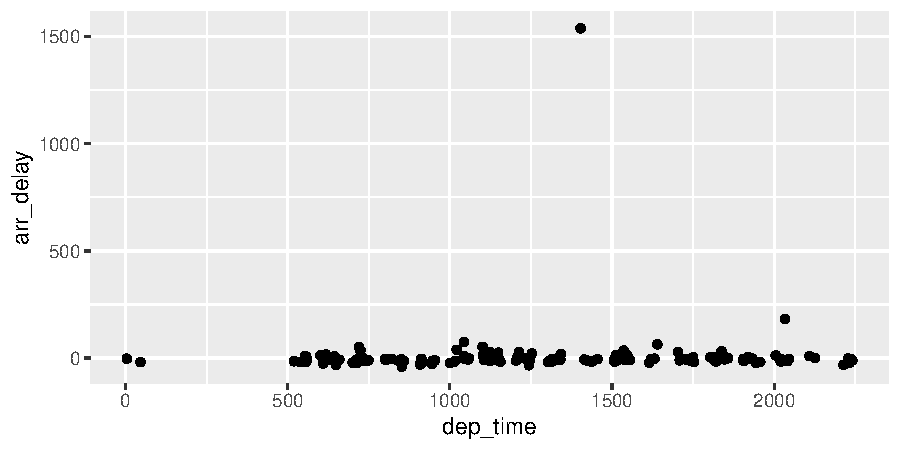
\includegraphics{firstName-lastName_StatThesis_files/figure-latex/march3plot-1} \end{center}
\begin{proof}[This is a proof]
There is a proof environment in which you can create equations

\[
\hat{\beta}_0 + \hat{\beta}_1x
\]
\end{proof}
\hypertarget{additional-resources}{%
\section{Additional resources}\label{additional-resources}}
\begin{itemize}
\item
  \emph{Markdown} Cheatsheet - \url{https://github.com/adam-p/markdown-here/wiki/Markdown-Cheatsheet}
\item
  \emph{R Markdown} Reference Guide - \url{https://www.rstudio.com/wp-content/uploads/2015/03/rmarkdown-reference.pdf}
\item
  Introduction to \texttt{dplyr} - \url{https://cran.rstudio.com/web/packages/dplyr/vignettes/introduction.html}
\item
  \texttt{ggplot2} Documentation - \url{http://docs.ggplot2.org/current/}
\end{itemize}
\hypertarget{math-sci}{%
\chapter{Mathematics and Science}\label{math-sci}}

\hypertarget{math}{%
\section{Math}\label{math}}

\TeX~is the best way to typeset mathematics. Donald Knuth designed \TeX~when he got frustrated at how long it was taking the typesetters to finish his book, which contained a lot of mathematics. One nice feature of \emph{R Markdown} is its ability to read LaTeX code directly.

If you are doing a thesis that will involve lots of math, you will want to read the following section.

\[
\sum_{j=1}^n (\delta\theta_j)^2 \leq 
\frac{\beta_i^2}{\delta_i^2 + \rho_i^2}
\left[ 2\rho_i^2 + \frac{\delta_i^2\beta_i^2}{\delta_i^2 + \rho_i^2} \right] \equiv \omega_i^2
\]

From Informational Dynamics, we have the following (Dave Braden):

After \emph{n} such encounters the posterior density for \(\theta\) is

\[
\pi(\theta|X_1< y_1,\dots,X_n<y_n) \varpropto \pi(\theta) \prod_{i=1}^n\int_{-\infty}^{y_i}
   \exp\left(-\frac{(x-\theta)^2}{2\sigma^2}\right)\ dx
\]

Another equation:

\[
\det\left|\,\begin{matrix}%
c_0&c_1\hfill&c_2\hfill&\ldots&c_n\hfill\cr
c_1&c_2\hfill&c_3\hfill&\ldots&c_{n+1}\hfill\cr
c_2&c_3\hfill&c_4\hfill&\ldots&c_{n+2}\hfill\cr
\,\vdots\hfill&\,\vdots\hfill&
  \,\vdots\hfill&&\,\vdots\hfill\cr
c_n&c_{n+1}\hfill&c_{n+2}\hfill&\ldots&c_{2n}\hfill\cr
\end{matrix}\right|>0
\]

\hypertarget{statistics-symbols-and-expressions}{%
\section{Statistics Symbols and Expressions}\label{statistics-symbols-and-expressions}}

\noindent Exponent or Superscript: \(x^2\)

\noindent Subscript: \(x_1, x_2, \dots, x_n\)

\noindent Both combined: \(x_1^{k+1}\).

\noindent Our favorite Greeks: \(\sigma\), \(\epsilon\), \(\mu\)

\noindent Defining a normally distributed random variable: \(X\sim N(\mu, \sigma)\)

How do we compute sample variance again?

\[s^2 = \frac{\sum_{i=1}^n (x_i-\bar x)^2}{n-1}\]

Sometimes you'll need to consider asymptotics, that is, what happens as \(n\rightarrow \infty\).

\hypertarget{additional-information}{%
\section{Additional information}\label{additional-information}}

Many of the symbols you will need can be found on Reed College's math page \url{http://web.reed.edu/cis/help/latex/math.html} and the Comprehensive LaTeX Symbol Guide (\url{http://mirror.utexas.edu/ctan/info/symbols/comprehensive/symbols-letter.pdf}).

\hypertarget{ref-labels}{%
\chapter{Tables, Graphics, References, and Labels}\label{ref-labels}}

\hypertarget{conclusion}{%
\chapter*{Conclusion}\label{conclusion}}
\addcontentsline{toc}{chapter}{Conclusion}

If we don't want the conclusion to have a chapter number next to it, we can add the \texttt{\{-\}} attribute.

\textbf{More info}

And here's some other random info: the first paragraph after a chapter title or section head \emph{shouldn't be} indented, because indents are to tell the reader that you're starting a new paragraph. Since that's obvious after a chapter or section title, proper typesetting doesn't add an indent there.

\appendix

\hypertarget{the-first-appendix}{%
\chapter{The First Appendix}\label{the-first-appendix}}

This first appendix includes all of the R chunks of code that were hidden throughout the document (using the \texttt{include\ =\ FALSE} chunk tag) to help with readibility and/or setup.

\hypertarget{in-the-main-file-refref-labels}{%
\section{In the main file \ref{ref-labels}:}\label{in-the-main-file-refref-labels}}

\hypertarget{in-chapter-refref-labels}{%
\section{In Chapter \ref{ref-labels}:}\label{in-chapter-refref-labels}}

\hypertarget{the-second-appendix}{%
\chapter{The Second Appendix}\label{the-second-appendix}}

R code

\hypertarget{corrections}{%
\chapter*{Corrections}\label{corrections}}
\addcontentsline{toc}{chapter}{Corrections}

A list of corrections after submission to department.

Corrections may be made to the body of the thesis, but every such correction will be acknowledged in a list under the heading ``Corrections,'' along with the statement ``When originally submitted, this honors thesis contained some errors which have been corrected in the current version. Here is a list of the errors that were corrected.'' This list will be given on a sheet or sheets to be appended to the thesis. Corrections to spelling, grammar, or typography may be acknowledged by a general statement such as ``30 spellings were corrected in various places in the thesis, and the notation for definite integral was changed in approximately 10 places.'' However, any correction that affects the meaning of a sentence or paragraph should be described in careful detail. The files samplethesis.tex and samplethesis.pdf show what the ``Corrections'' section should look like. Questions about what should appear in the ``Corrections'' should be directed to the Chair.

\backmatter

\hypertarget{references}{%
\chapter*{References}\label{references}}
\addcontentsline{toc}{chapter}{References}

\noindent

\setlength{\parindent}{-0.20in}
\setlength{\leftskip}{0.20in}
\setlength{\parskip}{8pt}

\hypertarget{refs}{}
\begin{CSLReferences}{1}{0}
\leavevmode\vadjust pre{\hypertarget{ref-angel2000}{}}%
Angel, E. (2000). \emph{Interactive computer graphics : A top-down approach with OpenGL}. Boston, MA: Addison Wesley Longman.

\leavevmode\vadjust pre{\hypertarget{ref-angel2001}{}}%
Angel, E. (2001a). \emph{Batch-file computer graphics : A bottom-up approach with QuickTime}. Boston, MA: Wesley Addison Longman.

\leavevmode\vadjust pre{\hypertarget{ref-angel2002a}{}}%
Angel, E. (2001b). \emph{Test second book by angel}. Boston, MA: Wesley Addison Longman.

\end{CSLReferences}
% Index?

\end{document}
